\subsection{Regulación de sistemas lineales: caso 3}

La planta tiene un integrador, es decir, un polo en el origen

\begin{figure}[h!]
    \centering
        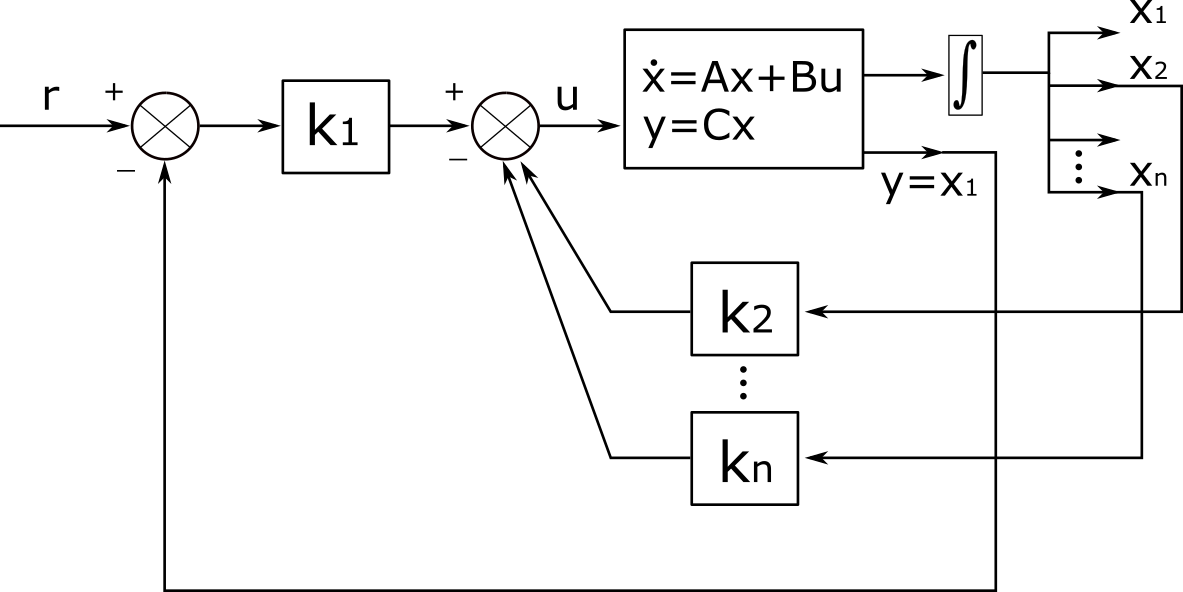
\includegraphics[scale=0.17]{Control de Sistemas Mecatronicos Figuras/16 Con integrador en la Planta.png}
        \caption{Sistema con integrador en la planta}
\end{figure}

Sea el sistema 
\[
    (1)
    \left\{
        \begin{array}{lll}
            \dot{x}(t) = Ax(t) + Bu(t) \\
            y(t) = Cx(t)
        \end{array}
    \right.
\]

La entrada del sistema es
\[
    \begin{split}
        u & = k_{1}(r - x_{1}) - k_{2}x_{2} - k_{3}x_{3} - \ldots - k_{n}x_{n} \\
        & = k_{1}r - k_{1}x_{1} - k_{2}x_{2} - k_{3}x_{3} - \ldots - k_{n}x_{n} \\
        & = k_{1}r - 
        \begin{bmatrix}
            k_{1} & k_{2} & \ldots & k_{n}
        \end{bmatrix}
        \begin{bmatrix}
            x_{1} \\ x_{2} \\ \vdots \\ x_{n}
        \end{bmatrix} \\
        & = k_{1}r - kx
    \end{split}
\]

\begin{figure}[h!]
    \centering
        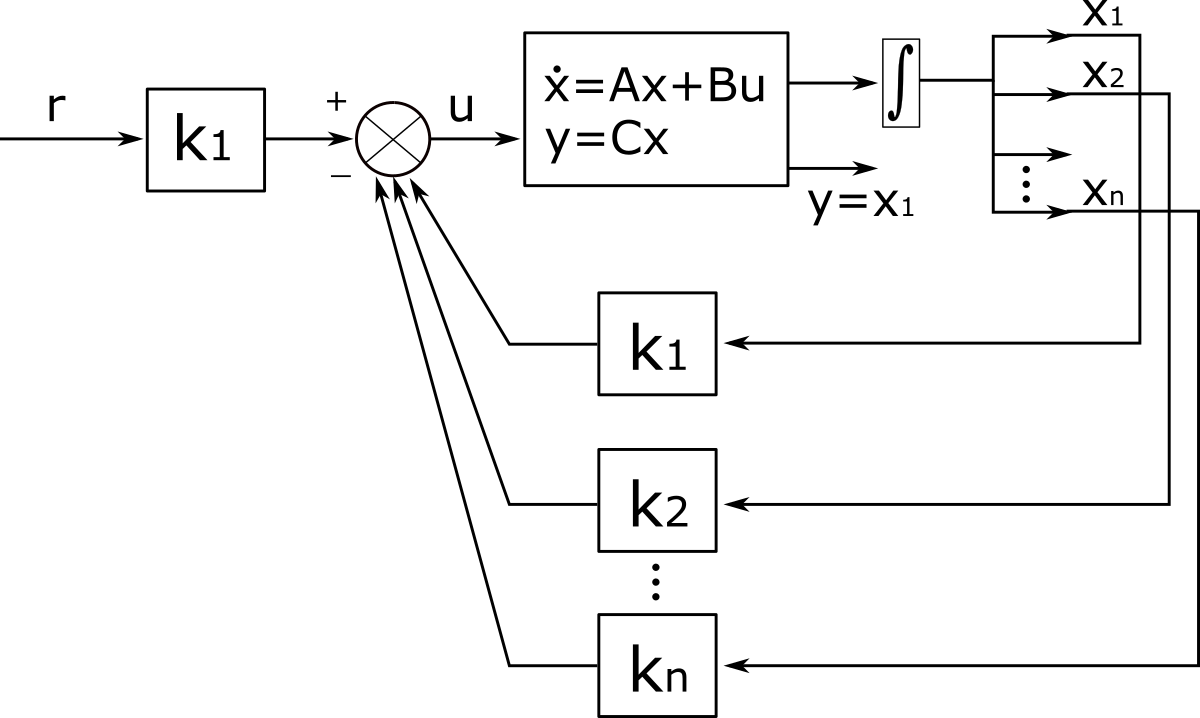
\includegraphics[scale=0.19]{Control de Sistemas Mecatronicos Figuras/17 Con integrador en la Planta.png}
        \caption{Sistema con integrador en la planta}
\end{figure}

Sustituyendo (2) en (1)
\[
    \begin{split}
        \dot{x} & = Ax + B(k_{1}r - kx) \\
        & = Ax + Bk_{1}r - Bkx \\
        & = (A-Bk)x + Bk_{1}r
    \end{split}
\]

El problema de regulación se resuelve como un problema de ubicación de polos para la matriz \( A-Bk \)